\subsection{Susannah Brook model v2 (model ID: 10)}
The Susannah Brook model v2 model (fig.~\ref{fig:10_schematic}) is part of a top-down modelling exercise designed to use auxiliary data \citep{Son2007}. It has 2 stores and 6 parameters ($S_b$, $\phi$, $fc$, $r$, $c$, $d$). For consistency with other model formulations, $S_b$ is is used as a parameter, instead of being broken down into its constitutive parts $D$ and $\phi$. The model aims to represent:

\begin{itemizecompact}
\item Separation of saturated zone and a variable-size unsaturated zone;
\item Evaporation from unsaturated and saturated zones;
\item Saturation excess and non-linear subsurface flow;
\item Deep groundwater recharge.
\end{itemizecompact}

\subsubsection{File names}
\begin{tabular}{@{}ll}
Model: &m\_10\_susannah2\_6p\_2s \\
Parameter ranges: &m\_10\_susannah2\_6p\_2s\_parameter\_ ranges \\
\end{tabular}

% Equations
\subsubsection{Model equations}

% Model layout figure
{ 																	% This ensures it doesn't warp text further down
\begin{wrapfigure}{l}{5cm}
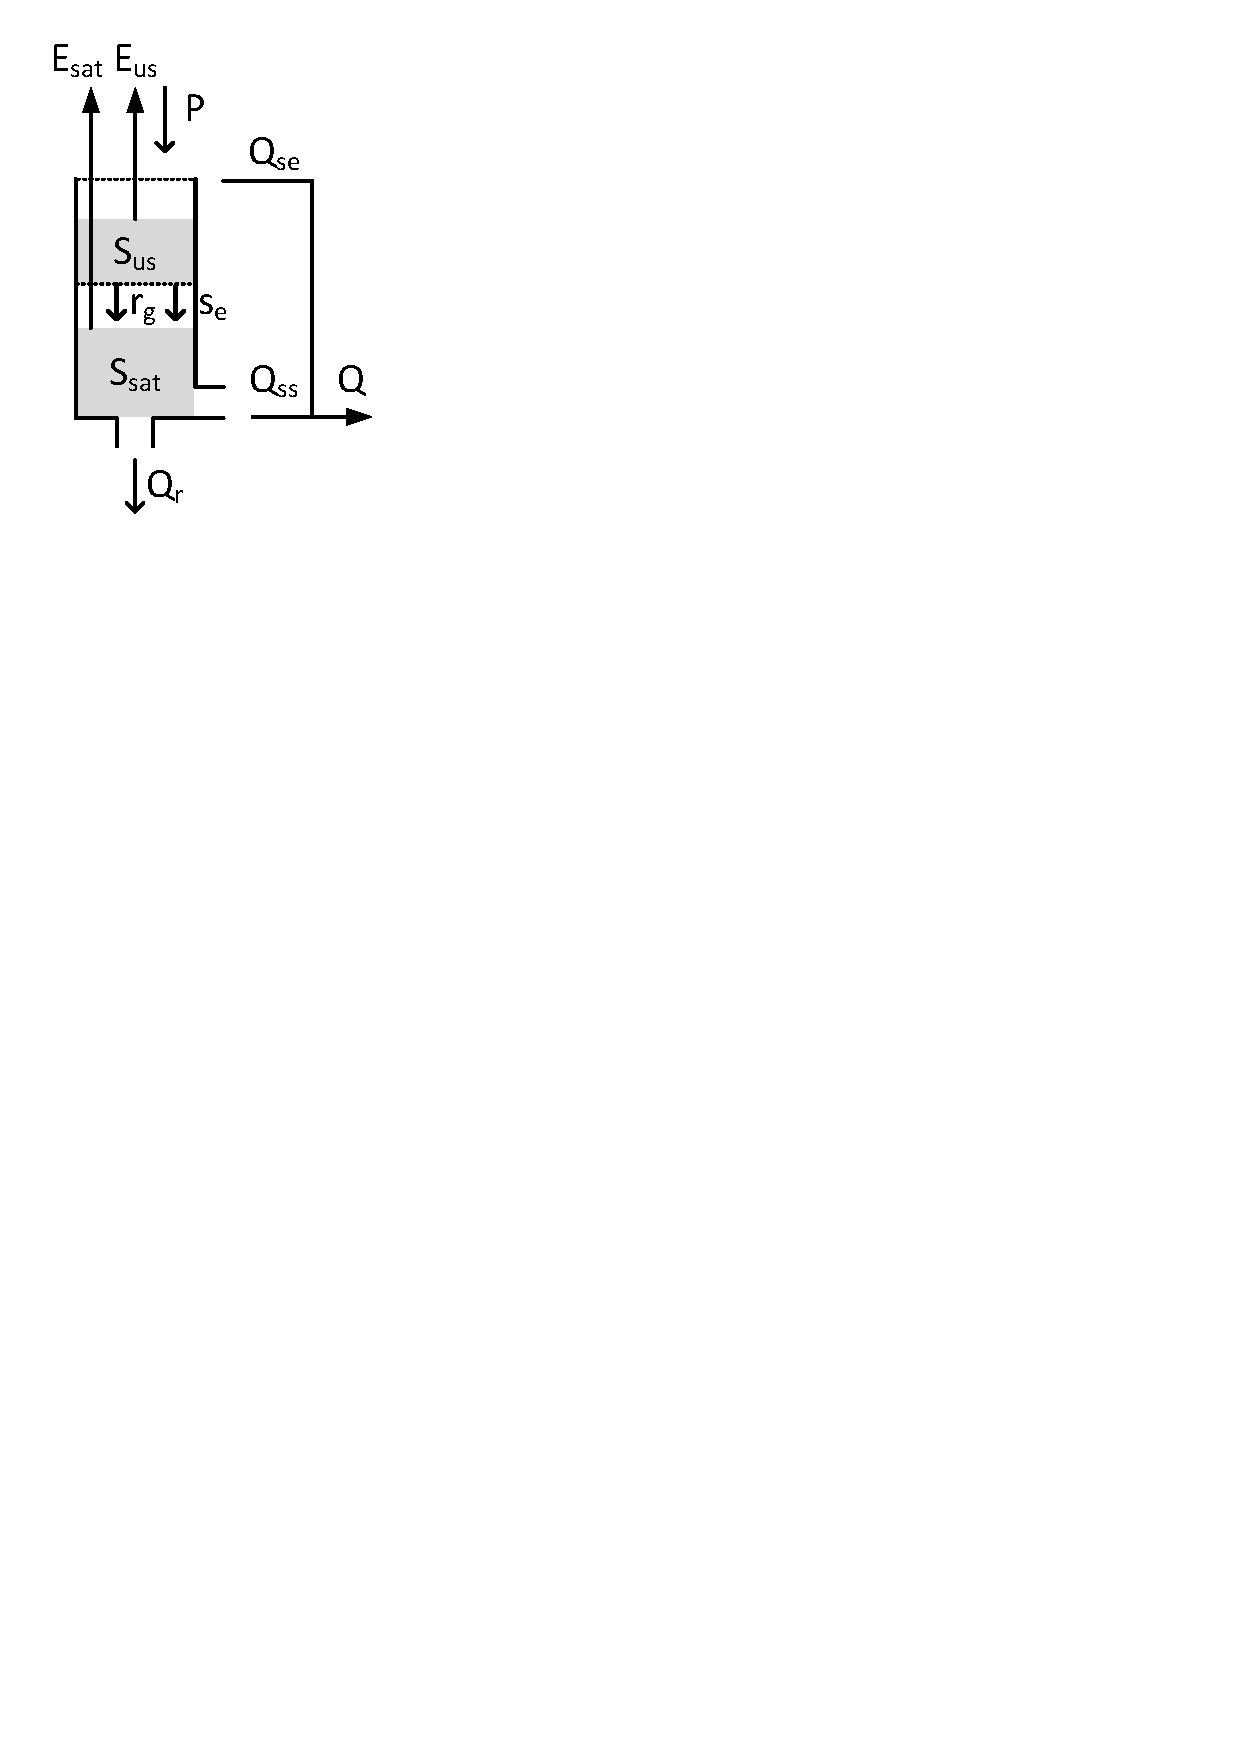
\includegraphics[trim=1cm 21cm 14cm 0.8cm,width=5cm,keepaspectratio]{./files/10_schematic.pdf}
\caption{Structure of the Susannah Brook v2 model} \label{fig:10_schematic}
\end{wrapfigure}

\begin{align}
	\frac{dS_{us}}{dt} &= P-E_{us}-r_g -S_e\\
	E_{us} &= \frac{S_{us}}{S_b}*E_p\\
	S_b &= D*\phi\\
	r_g &= 
	\begin{cases}
		P, & if~S_{us} > S_{usfc}\\
		0, & \text{otherwise} \\
	\end{cases} \\
	S_e &= \begin{cases}
			S_{us} - S_{usfc}, & if~S_{us} > S_{usfc}\\
			0, & \text{otherwise} \\
			\end{cases}\\
	S_{usfc} &= (S_b - S_{sat})*\frac{fc}{\phi} 
\end{align}

Where $S_{us}$ is the current storage in the unsaturated store [mm], $P$ the current precipitation [mm], $S_b$ [mm] the maximum storage of the soil profile, based on the soil depth $D$ [mm] and the porosity $\phi$ [-]. $r_g$ is drainage from the unsaturated store to the saturated store [mm], based on the variable field capacity $S_{usfc}$ [mm]. $S_{usfc}$ is based on the current storage on the saturated zone $S_{sat}$ [mm], the maximum soil moisture storage $S_b$ [mm], the field capacity $fc$ [-] and the porosity $\phi$ [-]. $S_e$ [mm] is the storage excess, resulting from a decrease of $S_{usfc}$ that leads to more water being stored in the unsaturated zone than should be possible.

} % end wrap

\begin{align}
	\frac{dS_{sat}}{dt} &= r_g - E_{sat} - Q_{SE} - Q_{SS} - Q_{R}\\
	E_{sat} &= \frac{S_{sat}}{S_b}*E_p\\
	Q_{SE} &= \begin{cases}
		r_g+S_e, &\text{if } S_{sat} > S_b \\
		0, & \text{otherwise} \\
	\end{cases} \\
	Q_{SS} &= (1-r)*c*\left(S_{sat}\right)^d\\
	Q_{R} &= r*c*\left(S_{sat}\right)^d
\end{align}

Where $S_{sat}$ is the current storage in the saturated zone [mm], $E_{sat}$ is the evaporation from the saturated zone [mm], $Q_{SE}$ saturation excess runoff [mm] that occurs when the saturated zone reaches maximum capacity $S_b$ [mm], $Q_{SS}$ is subsurface flow [mm] and $Q_R$ is recharge of deep groundwater [mm]. Both $Q_{SS}$ and $Q_R$ are based on the dimensionless fraction $r$ and subsurface flow constants $c$ $[d^{-1}]$ and $d$ [-]. Total runoff is the sum of $Q_{SE}$ and $Q_{SS}$:

\begin{align}
	Q &= Q_{SE} + Q_{SS}
\end{align}

\subsubsection{Parameter overview}
% Table generated by Excel2LaTeX from sheet 'Sheet1'
\begin{table}[htbp]
  \centering
    \begin{tabular}{lll}
    \toprule
    Parameter & Unit  & Description \\
    \midrule
    $S_b$ & $mm$  & Maximum soil moisture storage \\
    $\phi$ & $-$   & Porosity \\
    $fc$  & $-$   & Field capacity as fraction of $S_b$ \\
    $r$   & $-$   & Fraction of subsurface outflow to deep groundwater \\
    $c$   & $d^{-1}$ & Runoff coefficient \\
    $d$   & $-$   & Runoff nonlinearity \\
    \bottomrule
    \end{tabular}%
  \label{tab:addlabel}%
\end{table}%

